\section{Discussion and Outlook (1 page)}
\label{sec:discussion_outlook}
\begin{figure}[t]
\centering
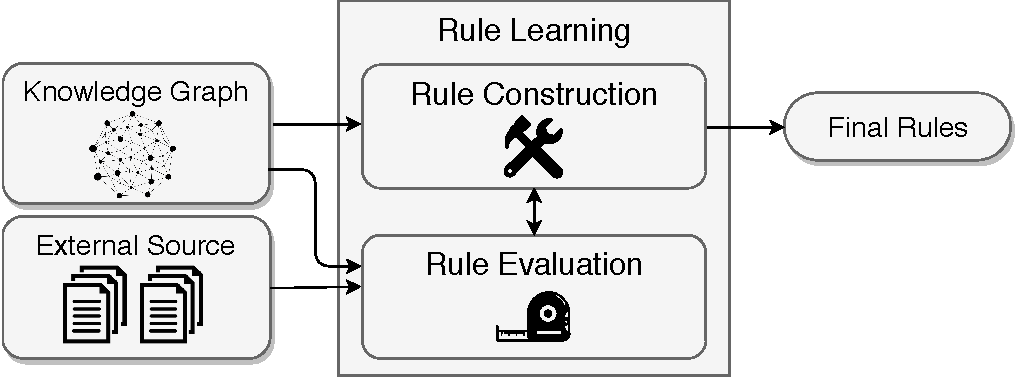
\includegraphics[width=8cm]{figures/discussion_overview}
\caption{Rule learning using external sources.}
\label{fig:discussion_overview}
\end{figure}
Toward the rule-based KG completion problem, a large number of rule learning systems have been proposed. While the rule construction methods of these systems may vary, the core of them is at the proposed rule evaluation metric. Various rule measures have been introduced, from the simplest to the most sophisticated one. Nevertheless, most of them are computed based on only the given graph, and cover only a small subset of local patterns in the KG, thus might wrongly estimate the quality of extracted rules since real-world KGs are usually highly incomplete.

One promising possibility to tackle this problem is to incorporate external related data from outside of the KG. This knowledge can be extracted from many sources (e.g. crowd-sourcing, Web-extraction), and is obviously useful not only for rule evaluation, but also for rule construction over the KG. For instance, external data can give some hints about the rules such as quality of predicted facts in form of probability/likelihood, give some information about the existence of certain types of facts within the KG (as exploited in CARL \cite{carl}).

Apart from rule learning approach, an alternative relational learning method for KG completion is to
learn representations (i.e. embeddings) of entities and relations for predicting likelihood of unseen facts. 
While these methods capture global patterns in the data, and can be extended with additional unstructured knowledge (e.g., text corpus) the predictions that they produce are not interpretable. This put a question on how to integrate this approach into the rule learning approach to deal with the mentioned issue.
